\documentclass[aspectratio=169,10pt]{beamer}

\usepackage[T1]{fontenc}
\usepackage[utf8]{inputenc}
\usepackage[english]{babel}
\usepackage{lmodern}
\usepackage{microtype}
\usepackage{amsmath}
\usepackage{booktabs}
\usepackage{csquotes}
\usepackage{graphicx}
\usepackage{pgfplots}
\usepackage{xcolor}
\usepackage{tikz}

\usetikzlibrary{arrows.meta,calc,fit,positioning}
\pgfplotsset{compat=1.18}

\definecolor{LanceNavy}{HTML}{123B5D}
\definecolor{LanceBlue}{HTML}{1F6F9F}
\definecolor{LanceCyan}{HTML}{1597A8}
\definecolor{LanceGreen}{HTML}{2E7D5B}
\definecolor{LanceOrange}{HTML}{D97721}
\definecolor{LanceRed}{HTML}{B64045}
\definecolor{LanceLight}{HTML}{F3F7FA}
\definecolor{LanceInk}{HTML}{263746}

\usetheme{default}
\usefonttheme{professionalfonts}
\setbeamertemplate{navigation symbols}{}
\setbeamersize{text margin left=7mm,text margin right=7mm}

\setbeamercolor{normal text}{fg=LanceInk,bg=white}
\setbeamercolor{structure}{fg=LanceBlue}
\setbeamercolor{frametitle}{fg=white,bg=LanceNavy}
\setbeamercolor{block title}{fg=white,bg=LanceBlue}
\setbeamercolor{block body}{fg=LanceInk,bg=LanceLight}
\setbeamercolor{block title alerted}{fg=white,bg=LanceOrange}
\setbeamercolor{block body alerted}{fg=LanceInk,bg=LanceOrange!10}
\setbeamercolor{block title example}{fg=white,bg=LanceGreen}
\setbeamercolor{block body example}{fg=LanceInk,bg=LanceGreen!9}
\setbeamercolor{author in head/foot}{fg=white,bg=LanceNavy}
\setbeamercolor{date in head/foot}{fg=white,bg=LanceBlue}

\setbeamerfont{frametitle}{series=\bfseries,size=\Large}
\setbeamerfont{title}{series=\bfseries,size=\LARGE}
\setbeamerfont{subtitle}{size=\large}
\setbeamerfont{block title}{series=\bfseries}

\setbeamertemplate{frametitle}{%
  \nointerlineskip
  \begin{beamercolorbox}[wd=\paperwidth,ht=3.0ex,dp=1.1ex,leftskip=7mm]{frametitle}
    \usebeamerfont{frametitle}\insertframetitle
  \end{beamercolorbox}
}

\setbeamertemplate{footline}{%
  \leavevmode
  \hbox{%
    \begin{beamercolorbox}[wd=.87\paperwidth,ht=2.7ex,dp=1.1ex,leftskip=7mm]{author in head/foot}
      \scriptsize Léo Basin \hspace{0.7em}--\hspace{0.7em} LANCE
    \end{beamercolorbox}%
    \begin{beamercolorbox}[wd=.13\paperwidth,ht=2.7ex,dp=1.1ex,center]{date in head/foot}
      \scriptsize\insertframenumber
    \end{beamercolorbox}%
  }
}

\newcommand{\reportlogo}[2][]{%
  \IfFileExists{squelette-latex/figures/#2}{%
    \includegraphics[#1]{squelette-latex/figures/#2}%
  }{%
    \includegraphics[#1]{metric/squelette-latex/figures/#2}%
  }%
}

\newcommand{\keymessage}[1]{%
  \begin{beamercolorbox}[rounded=true,sep=1.1ex,wd=\linewidth]{block body example}
    \centering\bfseries #1
  \end{beamercolorbox}
}

\tikzset{
  >={Latex[length=2.2mm]},
  flow/.style={->,semithick,draw=LanceInk!80},
  dashedflow/.style={->,semithick,dashed,draw=LanceOrange},
  box/.style={draw=LanceBlue,fill=LanceBlue!8,rounded corners=2pt,
    align=center,minimum height=8mm,inner sep=3pt,font=\scriptsize},
  greenbox/.style={draw=LanceGreen,fill=LanceGreen!9,rounded corners=2pt,
    align=center,minimum height=8mm,inner sep=3pt,font=\scriptsize},
  orangebox/.style={draw=LanceOrange,fill=LanceOrange!9,rounded corners=2pt,
    align=center,minimum height=8mm,inner sep=3pt,font=\scriptsize},
  phasebox/.style={draw=LanceCyan,fill=LanceCyan!9,rounded corners=2pt,
    align=center,minimum height=8mm,minimum width=18mm,inner sep=2pt,
    font=\scriptsize}
}

\title[HMoE and LANCE evaluation]{Designing an HMoE and evaluating LANCE}
\subtitle{An agentic \emph{Heterogeneous Mixture of Experts} for IoT/OT security auditing}
\author{Léo Basin}
\institute{TELECOM Nancy \quad--\quad University of Mons, ILIA Department}
\date{Second-year internship defence -- September 2026}

\begin{document}

% 0:30
{
  \setbeamercolor{background canvas}{bg=LanceNavy}
  \begin{frame}[plain]
    \color{white}
    \begin{columns}[c,onlytextwidth]
      \begin{column}{0.70\textwidth}
        {\usebeamerfont{title}\inserttitle\par}
        \vspace{0.4em}
        {\usebeamerfont{subtitle}\color{white!82}\insertsubtitle\par}
        \vspace{1.3em}
        {\large\bfseries Léo Basin}\par
        \vspace{0.25em}
        TELECOM Nancy -- second year\par
        University of Mons -- ILIA Department\par
        \vspace{0.9em}
        {\small Internship supervisor: Mr~Saïd Mahmoudi\par
        Academic supervisor: Mr~Thibault Cholez}
      \end{column}
      \begin{column}{0.27\textwidth}
        \centering
        \colorbox{white}{\reportlogo[width=0.78\linewidth]{university-logo.pdf}}\par
        \vspace{1em}
        \colorbox{white}{\reportlogo[width=0.78\linewidth]{school-logo.pdf}}
      \end{column}
    \end{columns}
    \vfill
    {\small\color{white!70}\insertdate}
  \end{frame}
}

\section{Context and research question}

% 1:00
\begin{frame}{Internship context and assignment}
  \begin{columns}[T,onlytextwidth]
    \begin{column}{0.47\textwidth}
      \begin{block}{Host institution}
        \begin{description}
          \item[Institution] University of Mons
          \item[Department] ILIA, Faculty of Engineering
          \item[Field] AI, IoT, distributed systems and cybersecurity
        \end{description}
      \end{block}
      \vspace{0.4em}
      \begin{exampleblock}{LANCE}
        LLM-based agent that conducts an IoT/OT network security audit in six
        phases, from topology analysis to the final report.
      \end{exampleblock}
    \end{column}
    \begin{column}{0.50\textwidth}
      \centering
      \resizebox{\linewidth}{!}{%
        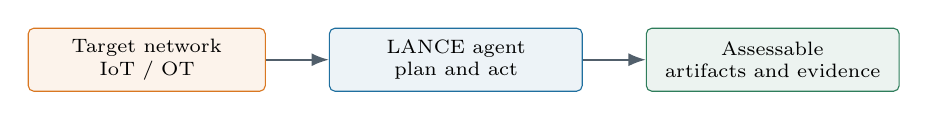
\begin{tikzpicture}[node distance=6mm]
          \node[orangebox,text width=28mm] (net) {Target network\\IoT / OT};
          \node[box,text width=30mm,right=8mm of net] (agent) {LANCE agent\\plan and act};
          \node[greenbox,text width=30mm,right=8mm of agent] (proof) {Assessable\\artifacts and evidence};
          \draw[flow] (net) -- (agent);
          \draw[flow] (agent) -- (proof);
        \end{tikzpicture}%
      }
      \vspace{1.2em}
      \begin{alertblock}{Main assignment}
        Specialise the local model for each audit role, integrate it into the
        pipeline, then make its behaviour measurable in reproducible scenarios.
      \end{alertblock}
    \end{column}
  \end{columns}
\end{frame}

% 1:00
\begin{frame}{Research question and motivation}
  \begin{alertblock}{Research question}
    \centering
    \large How can a local LLM agent be specialised for the different stages of
    an IoT/OT security audit, and how can the quality of its behaviour be
    demonstrated through a reproducible protocol?
  \end{alertblock}

  \vspace{0.6em}
  \begin{columns}[T,onlytextwidth]
    \begin{column}{0.32\textwidth}
      \begin{block}{Heterogeneous roles}
        Reconnaissance, analysis, exploitation and reporting require different
        tools and output contracts.
      \end{block}
    \end{column}
    \begin{column}{0.32\textwidth}
      \begin{block}{Generative outputs}
        A plausible or syntactically valid response may still be wrong or lack
        sufficient evidence.
      \end{block}
    \end{column}
    \begin{column}{0.32\textwidth}
      \begin{block}{Complex execution}
        A failure may come from the model, context, a tool or an ambiguous
        contract: its origin must remain identifiable.
      \end{block}
    \end{column}
  \end{columns}

  \vfill
  \keymessage{In this work, HMoE means \emph{Heterogeneous}, not \emph{Hierarchical Mixture of Experts}.}
\end{frame}

\section{Related work and architecture choices}

% 1:10
\begin{frame}{Related work: three specialisation strategies}
  \begin{columns}[T,onlytextwidth]
    \begin{column}{0.31\textwidth}
      \begin{block}{Prompt only}
        \textbf{Benefit:} no adaptation.\par
        \vspace{0.35em}
        \textbf{Limit:} long context and less stable roles.
      \end{block}
    \end{column}
    \begin{column}{0.31\textwidth}
      \begin{block}{One model per role}
        \textbf{Benefit:} strong isolation.\par
        \vspace{0.35em}
        \textbf{Limit:} duplicated weights and deployments.
      \end{block}
    \end{column}
    \begin{column}{0.34\textwidth}
      \begin{exampleblock}{Selected approach}
        One shared quantised base and four QLoRA adapters selected by a
        phase-based router.
      \end{exampleblock}
    \end{column}
  \end{columns}

  \vspace{0.7em}
  \begin{description}
    \item[QLoRA] Quantised weights remain frozen; only low-rank corrections are
      trained \cite{dettmers2023qlora}.
    \item[Neural MoE] A learned gate routes tokens between subnetworks
      \cite{shazeer2017moe}.
    \item[LANCE HMoE] A deterministic router selects one adapter for a complete
      request: heterogeneity lies in the roles.
  \end{description}
\end{frame}

% 1:10
\begin{frame}{LANCE: separating generation, execution and evaluation}
  \centering
  \resizebox{0.98\linewidth}{!}{%
    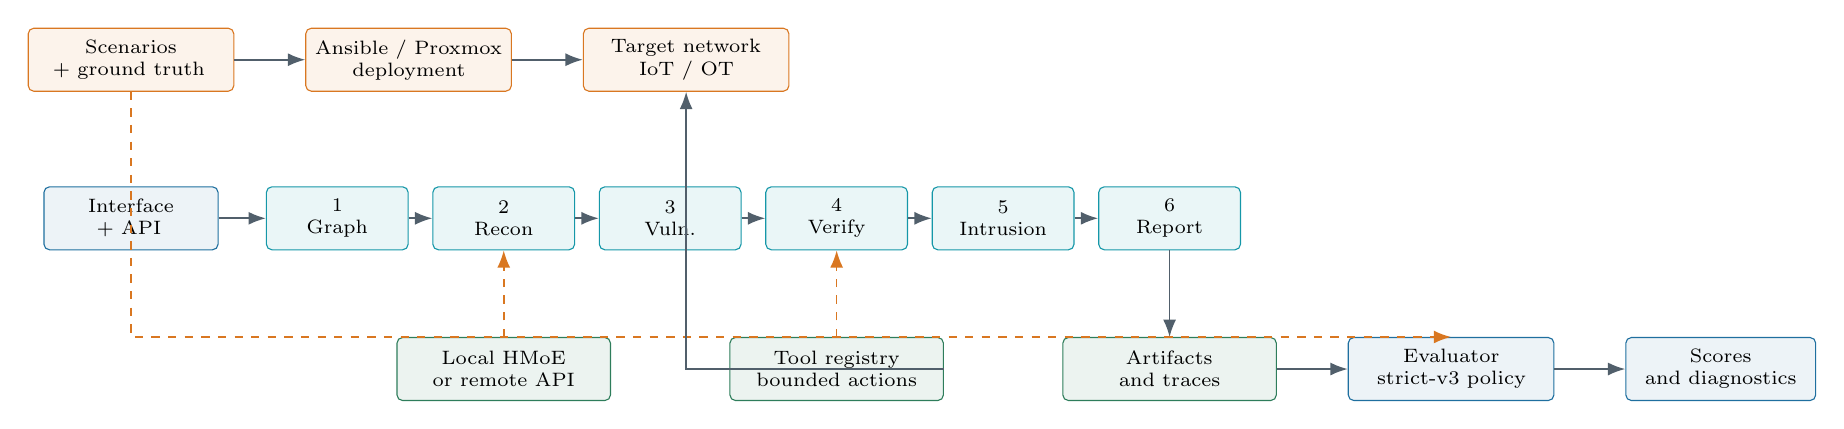
\begin{tikzpicture}[node distance=5mm]
      \node[orangebox,text width=24mm] (catalog) {Scenarios\\+ ground truth};
      \node[orangebox,text width=24mm,right=9mm of catalog] (deploy) {Ansible / Proxmox\\deployment};
      \node[orangebox,text width=24mm,right=9mm of deploy] (target) {Target network\\IoT / OT};
      \draw[flow] (catalog) -- (deploy);
      \draw[flow] (deploy) -- (target);

      \node[box,text width=20mm,below=12mm of catalog] (api) {Interface\\+ API};
      \node[phasebox,right=6mm of api] (p1) {1\\Graph};
      \node[phasebox,right=3mm of p1] (p2) {2\\Recon};
      \node[phasebox,right=3mm of p2] (p3) {3\\Vuln.};
      \node[phasebox,right=3mm of p3] (p4) {4\\Verify};
      \node[phasebox,right=3mm of p4] (p5) {5\\Intrusion};
      \node[phasebox,right=3mm of p5] (p6) {6\\Report};
      \draw[flow] (api) -- (p1);
      \draw[flow] (p1) -- (p2);
      \draw[flow] (p2) -- (p3);
      \draw[flow] (p3) -- (p4);
      \draw[flow] (p4) -- (p5);
      \draw[flow] (p5) -- (p6);

      \node[greenbox,text width=25mm,below=11mm of p2] (hmoe) {Local HMoE\\or remote API};
      \node[greenbox,text width=25mm,below=11mm of p4] (tools) {Tool registry\\bounded actions};
      \node[greenbox,text width=25mm,below=11mm of p6] (artifacts) {Artifacts\\and traces};
      \draw[dashedflow] (hmoe) -- (p2);
      \draw[dashedflow] (tools) -- (p4);
      \draw[flow] (p6) -- (artifacts);

      \node[box,text width=24mm,right=9mm of artifacts] (eval) {Evaluator\\strict-v3 policy};
      \node[box,text width=22mm,right=9mm of eval] (scores) {Scores\\and diagnostics};
      \draw[flow] (artifacts) -- (eval);
      \draw[flow] (eval) -- (scores);
      \draw[dashedflow] (catalog.south) |- (eval.north);
      \draw[flow] (tools.east) -| (target.south);
    \end{tikzpicture}%
  }

  \vspace{0.8em}
  \keymessage{The model proposes; the pipeline authorises and executes; the evaluator measures without exposing ground truth to the agent.}
\end{frame}

\section{Implemented solution}

% 1:20
\begin{frame}{QLoRA: specialising without duplicating the base}
  \begin{columns}[c,onlytextwidth]
    \begin{column}{0.62\textwidth}
      \centering
      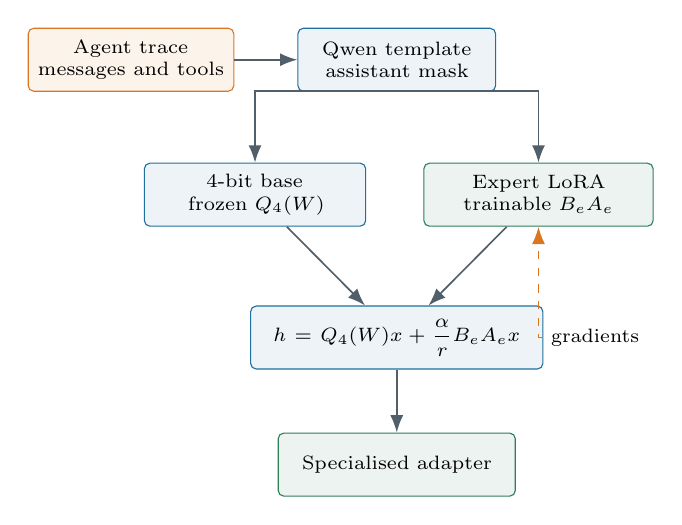
\begin{tikzpicture}[node distance=7mm]
        \node[orangebox,text width=24mm] (trace) {Agent trace\\messages and tools};
        \node[box,text width=23mm,right=8mm of trace] (template) {Qwen template\\assistant mask};
        \node[box,text width=26mm,below=9mm of template,xshift=-18mm] (base) {4-bit base\\frozen $Q_4(W)$};
        \node[greenbox,text width=27mm,below=9mm of template,xshift=18mm] (lora) {Expert LoRA\\trainable $B_eA_e$};
        \node[box,text width=35mm,below=10mm of base,xshift=18mm] (sum) {$h=Q_4(W)x+\dfrac{\alpha}{r}B_eA_ex$};
        \node[greenbox,text width=28mm,below=8mm of sum] (adapter) {Specialised adapter};
        \draw[flow] (trace) -- (template);
        \draw[flow] (template) -- ++(0,-4mm) -| (base);
        \draw[flow] (template) -- ++(0,-4mm) -| (lora);
        \draw[flow] (base) -- (sum);
        \draw[flow] (lora) -- (sum);
        \draw[flow] (sum) -- (adapter);
        \draw[dashedflow] (sum.east) -| node[pos=.25,right,font=\scriptsize]{gradients} (lora.south);
      \end{tikzpicture}
    \end{column}
    \begin{column}{0.35\textwidth}
      \begin{description}
        \item[Base] Qwen2.5-3B-Instruct, 4-bit NF4, BF16
        \item[LoRA] rank 16, $\alpha=32$, dropout $0.05$
        \item[Hardware] training within 16\,GiB of VRAM
      \end{description}
      \begin{alertblock}{Training context windows}
        6,144 tokens for secretary, reconnaissance and exploitation; 4,096 for
        the vulnerability expert, whose structured examples are shorter and
        remain untruncated at this limit.
      \end{alertblock}
    \end{column}
  \end{columns}
\end{frame}

% 1:20
\begin{frame}{Agentic HMoE: four roles, one shared base}
  \centering
  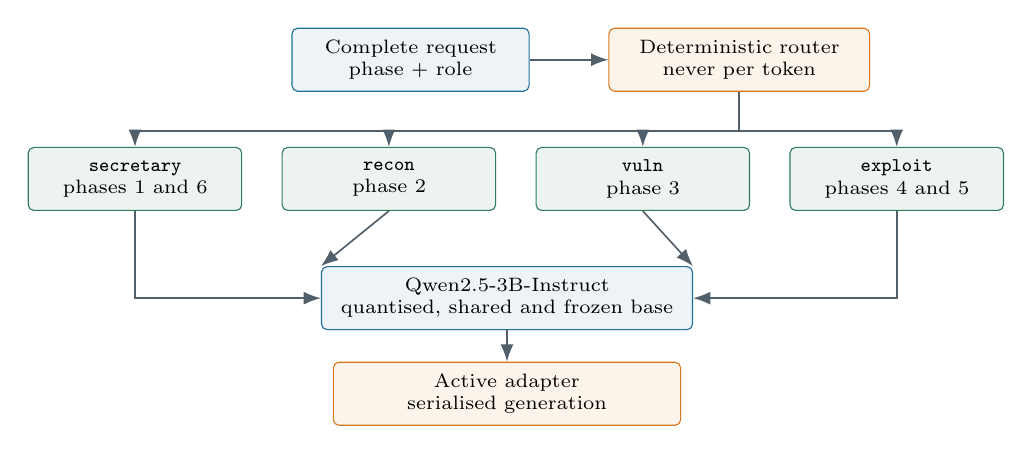
\begin{tikzpicture}[node distance=5mm]
    \node[box,text width=28mm] (request) {Complete request\\phase + role};
    \node[orangebox,text width=31mm,right=10mm of request] (router) {Deterministic router\\never per token};
    \draw[flow] (request) -- (router);

    \node[greenbox,text width=25mm,below=7mm of request,xshift=-35mm] (sec) {\texttt{secretary}\\phases 1 and 6};
    \node[greenbox,text width=25mm,right=5mm of sec] (recon) {\texttt{recon}\\phase 2};
    \node[greenbox,text width=25mm,right=5mm of recon] (vuln) {\texttt{vuln}\\phase 3};
    \node[greenbox,text width=25mm,right=5mm of vuln] (exploit) {\texttt{exploit}\\phases 4 and 5};

    \coordinate (split) at ($(router.south)+(0,-5mm)$);
    \draw[flow] (router.south) -- (split) -| (sec.north);
    \draw[flow] (split) -| (recon.north);
    \draw[flow] (split) -| (vuln.north);
    \draw[flow] (split) -| (exploit.north);

    \node[box,text width=45mm,below=7mm of recon,xshift=15mm] (base) {Qwen2.5-3B-Instruct\\quantised, shared and frozen base};
    \draw[flow] (sec.south) |- (base.west);
    \draw[flow] (recon.south) -- (base.north west);
    \draw[flow] (vuln.south) -- (base.north east);
    \draw[flow] (exploit.south) |- (base.east);

    \node[orangebox,text width=42mm,below=4mm of base] (lock) {Active adapter\\serialised generation};
    \draw[flow] (base) -- (lock);
  \end{tikzpicture}

  \vspace{0.1em}
  \footnotesize
  \begin{columns}[T,onlytextwidth]
    \begin{column}{0.49\textwidth}
      \begin{exampleblock}{Benefits}
        Interpretable routing, independent adapter replacement and only one copy
        of the base model.
      \end{exampleblock}
    \end{column}
    \begin{column}{0.49\textwidth}
      \begin{alertblock}{Trade-off}
        Experts are not combined; the lock protects adapter changes but
        serialises local inference.
      \end{alertblock}
    \end{column}
  \end{columns}
\end{frame}

% 1:00
\begin{frame}{From data sources to deployed experts}
  \begin{columns}[T,onlytextwidth]
    \begin{column}{0.55\textwidth}
      \small
      \begin{description}
        \item[Secretary] LANCE topologies, prompts and deliverables.
        \item[Reconnaissance] IoT-23 connection logs
          \cite{garcia2020iot23}.
        \item[Vulnerabilities] NIST NVD, CISA KEV and Exploit-DB mappings
          \cite{nistnvdapi,cisakev,offsecexploitdb}.
        \item[Exploitation] HackTricks, HTB write-ups and Nuclei templates
          \cite{hacktricksrepo,momenbaselhtb,zweilosechtb,nucleitemplates}.
      \end{description}
      \begin{alertblock}{Quality principle}
        Traces preserve tool-call/result pairs; campaign corrections enter the
        dataset only after human review.
      \end{alertblock}
    \end{column}
    \begin{column}{0.42\textwidth}
      \centering
      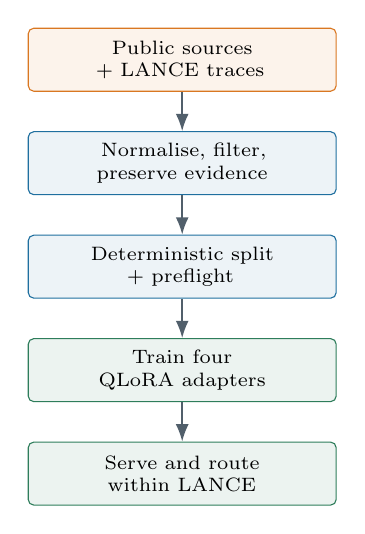
\begin{tikzpicture}[node distance=5mm]
        \node[orangebox,text width=37mm] (sources) {Public sources\\+ LANCE traces};
        \node[box,text width=37mm,below=of sources] (prepare) {Normalise, filter,\\preserve evidence};
        \node[box,text width=37mm,below=of prepare] (preflight) {Deterministic split\\+ preflight};
        \node[greenbox,text width=37mm,below=of preflight] (train) {Train four\\QLoRA adapters};
        \node[greenbox,text width=37mm,below=of train] (serve) {Serve and route\\within LANCE};
        \draw[flow] (sources) -- (prepare);
        \draw[flow] (prepare) -- (preflight);
        \draw[flow] (preflight) -- (train);
        \draw[flow] (train) -- (serve);
      \end{tikzpicture}
    \end{column}
  \end{columns}
\end{frame}

% 1:10
\begin{frame}{Beyond the model: pipeline and harness}
  \begin{columns}[T,onlytextwidth]
    \begin{column}{0.49\textwidth}
      \begin{block}{Strengthened pipeline}
        \begin{itemize}
          \item phase-specific contracts and authorised tools;
          \item structured artifacts and evidence registry;
          \item bounded recovery after a rejected deliverable;
          \item independent analyses parallelised when safe.
        \end{itemize}
      \end{block}
    \end{column}
    \begin{column}{0.49\textwidth}
      \begin{exampleblock}{Experimental harness}
        \begin{itemize}
          \item reproducible scenario deployment;
          \item ground truth retained by the evaluator;
          \item global one-to-one finding matching;
          \item fail-closed handling of incompatible contracts or artifacts.
        \end{itemize}
      \end{exampleblock}
    \end{column}
  \end{columns}

  \vspace{0.7em}
  \keymessage{The harness is the experimental system; \texttt{strict-v3} is the scoring policy applied by its evaluator.}
\end{frame}

\section{Evaluation and results}

% 1:15
\begin{frame}{Measuring a finding that is both correct and supported}
  \begin{columns}[T,onlytextwidth]
    \begin{column}{0.55\textwidth}
      For each retained match $i$:
      \[
        q_i=a_i\,s_i\,v_i, \qquad \mathrm{QTP}=\sum_i q_i
      \]
      \[
        P_Q=\frac{\mathrm{QTP}}{\mathrm{TP}+\mathrm{FP}},\quad
        R_Q=\frac{\mathrm{QTP}}{N_{\mathrm{GT}}},\quad
        Q\text{-}F_1=\frac{2P_QR_Q}{P_Q+R_Q}
      \]
      \[
        H=\frac{\mathrm{FP}}{\mathrm{TP}+\mathrm{FP}}
      \]
      \scriptsize $a_i$: matching quality; $s_i$: severity accuracy; $v_i$:
      evidence quality. Here, $H$ measures findings with no ground-truth match,
      not every possible form of semantic hallucination.
    \end{column}
    \begin{column}{0.42\textwidth}
      \begin{block}{Experimental snapshot}
        \begin{description}
          \item[Campaigns] 94 evaluable runs from August 2026
          \item[Scenarios] S1 to S11
          \item[Configurations] \texttt{lance-moe} and MiniMax-M2.7
          \item[Analysis] means + detailed traces from 11 August
        \end{description}
      \end{block}
      \begin{alertblock}{Interpretation limit}
        Repetitions and versions are unbalanced: these are descriptive results,
        not a causal model comparison.
      \end{alertblock}
    \end{column}
  \end{columns}
\end{frame}

% 2:00
\begin{frame}{August results: where does \texttt{lance-moe} degrade?}
  \begin{columns}[c,onlytextwidth]
    \begin{column}{0.62\textwidth}
      \centering
      \begin{tikzpicture}
        \begin{axis}[
          width=\linewidth,
          height=0.66\textheight,
          xmin=0.20,xmax=0.85,
          ymin=-0.02,ymax=0.62,
          xlabel={Mean Q-F1 $\rightarrow$},
          ylabel={Mean hallucination rate},
          grid=major,
          axis lines=left,
          tick label style={font=\scriptsize},
          label style={font=\small},
          clip=false
        ]
          \path[fill=LanceGreen!9] (axis cs:0.55,-0.02) rectangle (axis cs:0.85,0.20);
          \node[font=\scriptsize,text=LanceGreen!70!black,anchor=south east]
            at (axis cs:0.84,0.02) {target region};

          \addplot[only marks,mark=*,mark size=2.4pt,LanceBlue]
            coordinates {(0.474,0.209) (0.538,0.111) (0.505,0.163)
              (0.448,0.134) (0.528,0.125) (0.334,0.267) (0.491,0.389)};
          \addplot[only marks,mark=*,mark size=3pt,LanceGreen]
            coordinates {(0.611,0.000) (0.796,0.000)};
          \addplot[only marks,mark=*,mark size=3pt,LanceRed]
            coordinates {(0.281,0.556) (0.270,0.438)};

          \node[font=\scriptsize,anchor=south] at (axis cs:0.611,0.000) {S1};
          \node[font=\scriptsize,anchor=south] at (axis cs:0.796,0.000) {S9};
          \node[font=\scriptsize,anchor=north east] at (axis cs:0.474,0.209) {S2};
          \node[font=\scriptsize,anchor=west] at (axis cs:0.281,0.556) {S3};
          \node[font=\scriptsize,anchor=east] at (axis cs:0.538,0.111) {S4};
          \node[font=\scriptsize,anchor=south] at (axis cs:0.505,0.163) {S5};
          \node[font=\scriptsize,anchor=north east] at (axis cs:0.448,0.134) {S6};
          \node[font=\scriptsize,anchor=west] at (axis cs:0.528,0.125) {S7};
          \node[font=\scriptsize,anchor=west] at (axis cs:0.270,0.438) {S8};
          \node[font=\scriptsize,anchor=south] at (axis cs:0.334,0.267) {S10};
          \node[font=\scriptsize,anchor=west] at (axis cs:0.491,0.389) {S11};
        \end{axis}
      \end{tikzpicture}
    \end{column}
    \begin{column}{0.36\textwidth}
      \begin{exampleblock}{Clearest results}
        S9 followed by S1 combine high Q-F1 with zero hallucination for
        \texttt{lance-moe}.
      \end{exampleblock}
      \begin{alertblock}{Observed degradation}
        S3 and S8 combine low Q-F1 with many false positives. S8 also introduces
        pivots across IT, IoT and OT zones.
      \end{alertblock}
      \scriptsize
      S2 and S5 are intermediate: protocol switching for S2, and similar findings
      to distinguish and connect for S5. S11 shows how a broad attack surface
      increases omissions and opportunities for execution failures.
    \end{column}
  \end{columns}
\end{frame}

\section{Conclusion}

% 0:55
\begin{frame}{Conclusion: answering the research question}
  \begin{columns}[T,onlytextwidth]
    \begin{column}{0.49\textwidth}
      \begin{exampleblock}{Specialise}
        One quantised local base is shared by four QLoRA adapters. The phase
        router activates the required role without duplicating the model.
      \end{exampleblock}
    \end{column}
    \begin{column}{0.49\textwidth}
      \begin{exampleblock}{Demonstrate quality}
        The pipeline makes actions and evidence traceable; the harness repeats
        scenarios and measures Q-F1, hallucination and completion.
      \end{exampleblock}
    \end{column}
  \end{columns}

  \vspace{0.8em}
  \begin{block}{What the internship establishes}
    Operational HMoE integration and a protocol that reveals where a campaign
    degrades: detection, evidence or attack-path construction.
  \end{block}

  \begin{alertblock}{What remains to be established}
    Current campaigns do not yet demonstrate a causal advantage over a general
    model, nor consistently verified attack paths.
  \end{alertblock}
\end{frame}

% 0:55
\begin{frame}{Research perspectives}
  \begin{columns}[T,onlytextwidth]
    \begin{column}{0.32\textwidth}
      \begin{block}{Hierarchical routing}
        Keep phase-level selection, then choose a sub-expert by vulnerability
        family in phase 4 or by action type in phase 5.
      \end{block}
    \end{column}
    \begin{column}{0.32\textwidth}
      \begin{block}{Parallel inference}
        Use several replicas or expert services to move beyond current
        serialisation while respecting dependencies and locks.
      \end{block}
    \end{column}
    \begin{column}{0.32\textwidth}
      \begin{block}{Future models}
        Retrain the adapters on a newer compact base, or evaluate distinct models
        per role through separate services.
      \end{block}
    \end{column}
  \end{columns}

  \vfill
  \keymessage{Move from heterogeneous roles to finer specialisation without losing reproducible evaluation.}
\end{frame}

% -----------------------------------------------------------------------------
% Backup slides for the discussion with the panel
% -----------------------------------------------------------------------------
\appendix

\begin{frame}{Backup: datasets and training}
  \centering
  \small
  \begin{tabular}{lrrr}
    \toprule
    Expert & Examples & Context & Evaluation loss \\
    \midrule
    Secretary & 19\,065 & 6\,144 & 0.0421 \\
    Reconnaissance & 9\,257 & 6\,144 & 0.2102 \\
    Vulnerabilities & 6\,951 & 4\,096 & 0.00475 \\
    Exploitation & 14\,629 & 6\,144 & 0.00836 \\
    \bottomrule
  \end{tabular}

  \vspace{1em}
  \begin{alertblock}{Correct interpretation}
    Losses cannot be compared directly between experts: sequence lengths,
    format repetition and output diversity differ. They indicate convergence,
    not the operational effectiveness of the HMoE.
  \end{alertblock}
\end{frame}

\begin{frame}{Backup: three levels of success}
  \centering
  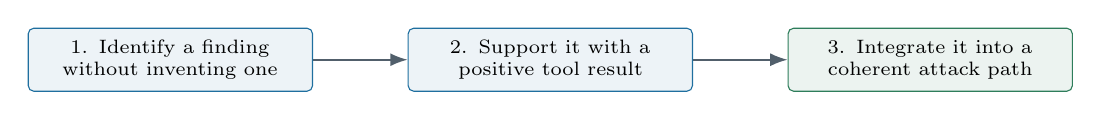
\begin{tikzpicture}[node distance=12mm]
    \node[box,text width=34mm] (finding) {1. Identify a finding\\without inventing one};
    \node[box,text width=34mm,right=of finding] (proof) {2. Support it with a\\positive tool result};
    \node[greenbox,text width=34mm,right=of proof] (path) {3. Integrate it into a\\coherent attack path};
    \draw[flow] (finding) -- (proof);
    \draw[flow] (proof) -- (path);
  \end{tikzpicture}

  \vspace{1.2em}
  \begin{description}
    \item[Hallucination rate] primarily describes the first level.
    \item[Q-F1] reflects matching, severity and evidence quality.
    \item[Verified F1 / paths] requires traceable evidence and, for a path, the
      correct ordering of devices.
  \end{description}

  \begin{alertblock}{Observation from 11 August}
    In the detailed \texttt{lance-moe} runs, no path was fully verified:
    evidence continuity between phases remains a priority.
  \end{alertblock}
\end{frame}

\begin{frame}{Backup: proposed ablation protocol}
  \begin{enumerate}
    \item base model with prompt only;
    \item one global QLoRA adapter trained on the combined dataset;
    \item four experts with the correct role selected explicitly;
    \item HMoE with automatic routing;
    \item deliberate permutation of selected experts to verify that any gain
      comes from specialisation rather than additional parameters alone.
  \end{enumerate}

  \vspace{0.8em}
  \keymessage{Same scenarios, tools and generation budgets, with balanced repetitions.}
\end{frame}

\begin{frame}[allowframebreaks]{References}
  \scriptsize
  \begin{thebibliography}{99}
    \bibitem{dettmers2023qlora}
      T.~Dettmers, A.~Pagnoni, A.~Holtzman and L.~Zettlemoyer.
      \newblock \emph{QLoRA: Efficient Finetuning of Quantized LLMs}.
      \newblock NeurIPS, 2023.

    \bibitem{shazeer2017moe}
      N.~Shazeer et al.
      \newblock \emph{Outrageously Large Neural Networks: The Sparsely-Gated
      Mixture-of-Experts Layer}.
      \newblock ICLR, 2017.

    \bibitem{garcia2020iot23}
      S.~Garcia, A.~Parmisano and M.~J.~Erquiaga.
      \newblock \emph{IoT-23: A Labeled Dataset with Malicious and Benign IoT
      Network Traffic}, 2020.

    \bibitem{nistnvdapi}
      National Institute of Standards and Technology.
      \newblock \emph{National Vulnerability Database: Vulnerabilities API 2.0}.

    \bibitem{cisakev}
      Cybersecurity and Infrastructure Security Agency.
      \newblock \emph{Known Exploited Vulnerabilities Catalog}.

    \bibitem{offsecexploitdb}
      OffSec.
      \newblock \emph{Exploit Database}.

    \bibitem{hacktricksrepo}
      HackTricks contributors.
      \newblock \emph{HackTricks}.

    \bibitem{momenbaselhtb}
      momenbasel contributors.
      \newblock \emph{HTB Writeups}.

    \bibitem{zweilosechtb}
      zweilosec.
      \newblock \emph{HTB Writeups}.

    \bibitem{nucleitemplates}
      ProjectDiscovery.
      \newblock \emph{Nuclei Templates}.
  \end{thebibliography}
\end{frame}

\end{document}
